\documentclass[UTF8,a4paper,12pt,titlepage,oneside]{ctexbook}
\usepackage{amsmath, amsthm, amssymb, bm, graphicx, geometry, mathrsfs, float, xcolor, fancyhdr}
\usepackage[colorlinks, linkcolor=black]{hyperref} % 超链接
\usepackage{subcaption}

\usepackage{listings}		% 为了避免与页眉的兼容问题可将listings放入table环境中
\lstset{
    basicstyle          =   \sffamily,          % 基本代码风格
    keywordstyle        =   \color{blue},          % 关键字风格
    keywordstyle    =   [2] \color{teal},
    commentstyle        =   \rmfamily\itshape,  % 注释的风格,斜体
    stringstyle         =   \ttfamily,  % 字符串风格
    flexiblecolumns,                % 别问为什么,加上这个
    numbers             =   left,   % 行号的位置在左边
    showspaces          =   false,  % 是否显示空格,显示了有点乱,所以不现实了
    numberstyle         =   \zihao{-5}\ttfamily,    % 行号的样式,小五号,tt等宽字体
    showstringspaces    =   false,
    captionpos          =   t,      % 这段代码的名字所呈现的位置,t指的是top上面
    frame               =   lrtb,   % 显示边框
    basicstyle          =   \zihao{-4}\ttfamily,
    stringstyle         =   \color{magenta},
    commentstyle        =   \color{red}\ttfamily,
    breaklines          =   true,   % 自动换行,建议不要写太长的行
    columns             =   fixed,  % 如果不加这一句,字间距就不固定,很丑,必须加
    basewidth           =   0.5em,
}
%% configure
\pagestyle{fancy}
\lhead{} 
\chead{\textit{\leftmark}} 
\rhead{} 
\lfoot{} 
\cfoot{\thepage}
\rfoot{}
\renewcommand\headrulewidth {0pt} 

\geometry{left=2.54cm, right=2.54cm, top=2.18cm, bottom=2.18cm}

\ctexset{
	chapter={
		format=\huge\bf\heiti\centering,
		number=\arabic{chapter},
		name={,},
		beforeskip={0pt},  % 设置章标题前面距离
		afterskip={18pt},   % 设置章标题后面距离
	}	
}

\begin{document}

% 目录

\newpage
\thispagestyle{empty}
\pagenumbering{roman}
\tableofcontents


%%  begin

\newpage
\setcounter{secnumdepth}{-1}
\setcounter{page}{1}
\pagenumbering{arabic}

\setcounter{chapter}{0}
\vspace{-3cm}\chapter{预备知识:通过键盘输入和文件输入}

\section{0.1 题目}
请自行敲代码练习Scanner 类接收键盘输入数据的模式。并通过 Java API 的查找发现 Scanner 与输入有关的其他函数,并加以验证练习。

\section{0.2 结果展示}
预备题较简单,完全为了熟悉Scanner的语法服务,代码附于附录。

\begin{figure}[H]
    \centering
    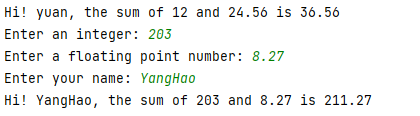
\includegraphics[width = 0.5\textwidth]{../pic/0.png}
    \caption{Problem0}
\end{figure}


\vspace{-3cm}\chapter{题目1:创建一个用来表示时间的类}

\section{1.1 题目}
\begin{enumerate}
    \item 创建一个用来存储时间数据的\lstinline{MyTime}类类型,当创建完这个类以后,应该保证下面的测试程序可以运行,且运行的结果如图所示。
    \begin{lstlisting}[
        language = Java,
        caption = {src/hw2/p1/TestTime.java, L5-L31}]
        // Official Test
        MyTime t1 = new MyTime();
        MyTime t2 = new MyTime(2);
        MyTime t3 = new MyTime(21, 34);
        MyTime t4 = new MyTime(12, 25, 42);
        MyTime t5 = new MyTime(t4);

        System.out.println("Constructed with:");
        System.out.println("t1: all arguments defaulted");
        System.out.printf(" %s\n", t1.toUniversalString());
        System.out.printf(" %s\n", t1.toString());
        System.out.println("t2: hour specified; minute and second defaulted");
        System.out.printf(" %s\n", t2.toUniversalString());
        System.out.printf(" %s\n", t2.toString());
        System.out.println("t3: hour and minute specified; second defaulted");
        System.out.printf(" %s\n", t3.toUniversalString());
        System.out.printf(" %s\n", t3.toString());
        System.out.println("t4: hour, minute and second specified");
        System.out.printf(" %s\n", t4.toUniversalString());
        System.out.printf(" %s\n", t4.toString());
        System.out.println("t5: MyTime object t4 specified");
        System.out.printf(" %s\n", t5.toUniversalString());
        System.out.printf(" %s\n", t5.toString());
        // when initialize t6 with invalid values,please output error information
        MyTime t6 = new MyTime(15, 74, 99);
        System.out.println("t6: invalid values");
        System.out.printf("%s\n", t6.toUniversalString());
    \end{lstlisting}
    \begin{figure}[H]
        \centering
        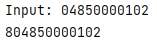
\includegraphics[width = 0.5\textwidth]{../pic/1/1.1.png}
        \caption{运行结果样例}
    \end{figure}
    \item 为\lstinline{MyTime}类增加三个成员方法:
    \begin{lstlisting}[language = Java]
    public void incrementHour();
    public void incrementMinute();
    public void incrementSecond();
    \end{lstlisting}
    每个方法都是在原有的对应数据上进行加1操作,但是一定要注意这种对时间的加1操作的合法性,比如考虑如下场景:\lstinline{MyTime}对象
    中的\lstinline{second}值为59,
    此时调用\lstinline{incrementSecond()}方法之后,\lstinline{second}值会成为0,同时\lstinline{minute}值也应该加1。
    将所有的特殊情况都考虑全面,并给出测试类。
\end{enumerate}


\section{1.2 题目分析}

本题需要对着已有的测试设计编写\lstinline{MyTime}类,并对\lstinline{increment}系列函数编写测试。

\begin{itemize}
    \item \textbf{Field}. 参照代码注释可知,可以定义三个\lstinline{int}变量\lstinline{hour}
        ,\lstinline{minute},\lstinline{second}分别代表小时、分钟、秒钟,24小时制。
    \item \textbf{Constructor Method}. 测试代码中一共出现了5种构造方法
    \begin{itemize}
        \item \lstinline{MyTime()},\lstinline{MyTime(int)},\lstinline{MyTime(int, int)},
        \lstinline{MyTime(int, int, int)};这4种构造方法都是直接将参数赋给类的变量,分别为
        默认、只赋时钟、只赋分钟、全赋值,未赋值的变量默认值为0;
        \item \lstinline{MyTime(MyTime)}这一构造方法是将参量复制给新的对象,即复制参量中的三个变量给新的对象。
        \item 值得注意的是,除了默认的构造方法外,构造方法均可以通过调用其他的构造方法实现,这样可以极大减少代码量,提高代码复用性。
    \end{itemize}
    \item \textbf{Other Method}. 本题目共要求实现编写5个实例化方法
    \begin{itemize}
        \item \lstinline{String toUniversalString()}. 本方法需要先判断\lstinline{this}数据是否合法,根据判断结果返回相应的字符串。
        \begin{enumerate}
            \item 判断\lstinline{this}的数据是否合法,因为错误信息需要检查所有的数据,所以设置一个初值为
                \lstinline{true}的\lstinline{boolean}变量\lstinline{flag},在判断过程中任一的判断错误
                都要将\lstinline{flag}置为\lstinline{false}.
            \item 如果不合法,输出判断过程中生成的错误信息
            \item 如果合法,根据\lstinline{this}的数据输出时间信息。此处需要注意字符串的输出格式:前导空格和Java format中的\lstinline{%02d}. 
        \end{enumerate}
        \item \lstinline{String toString()}. 本方法只需返回12小时制的时间字符串,所以只需注意\lstinline{hour}数据的处理和格式问题。
        \begin{enumerate}
            \item 参看测试代码可知,如果\lstinline{hour%12}为0,我们需要输出为12点,其他情况取余即可
            \item 格式问题可以参照上一个方法中的第三条,并在最后附上\lstinline{AM}/\lstinline{PM}
        \end{enumerate}
        \item \lstinline{increment}系列方法. 这几个方法逻辑基本类似,都是判断数据\lstinline{++}后是否超过上界,如果越界了需要将该数据置为0,
        并将更高级的单位数据\lstinline{++}。
        \begin{itemize}
            \item 基于这种\lstinline{++}操作的传递性,我们可以通过调用上一级单位的\lstinline{increment}方法简化我们的代码逻辑。
        \end{itemize}
    \end{itemize}
    \item \textbf{Test for Increment}. 测试代码只需确定每个\lstinline{increment}函数都正确无误,并测试其易错的进位即可,根据这个思路设计
        \lstinline{01:02:03}和\lstinline{23:59:59}. 
    两个数据。
    
\end{itemize}

\section{1.3 结果展示}

\begin{figure}[H]
    \centering
    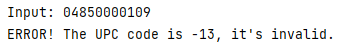
\includegraphics[width = 0.5\textwidth]{../pic/1/1.4.png}
    \caption{运行结果}
\end{figure}

\section{1.4 主干代码}

\begin{lstlisting}[
    language = Java,
    caption = {MyTime.java L8-L87}]
    public class MyTime {
    int hour;
    int minute;
    int second;

    MyTime() {
        hour = 0;
        minute = 0;
        second = 0;
    }

    MyTime(int h) {
        this();
        hour = h;
    }

    public MyTime(int h, int m) {
        this(h);
        minute = m;
    }

    public MyTime(int h, int m, int s) {
        this(h, m);
        second = s;
    }

    public MyTime(MyTime t4) {
        this(t4.hour, t4.minute, t4.second);
    }

    boolean ValidJudge(int num) {
        return num < 0 || num >= 60;
    }

    public String toUniversalString() {
        boolean flag = true;
        String s = "";

        if (ValidJudge(hour)) {
            flag = false;
            s += "hour must be 0-23\n";
        }
        if (ValidJudge(minute)) {
            flag = false;
            s += "minute must be 0-59\n";
        }
        if (ValidJudge(second)) {
            flag = false;
            s += "second must be 0-59\n";
        }
        if (flag) return String.format("   %02d:%02d:%02d", hour, minute, second);
        else return s;
    }

    @Override
    public String toString() {
        String s;
        s = (hour % 12 == 0) ? String.format("   %02d:%02d:%02d ", 12, minute, second) :
                String.format("   %02d:%02d:%02d ", hour % 12, minute, second);
        s += (hour < 12) ? "AM" : "PM";
        return s;
    }

    public void incrementHour() {
        if (++hour >= 24) hour = 0;
    }

    public void incrementMinute() {
        if (++minute >= 60) {
            minute = 0;
            incrementHour();
        }
    }

    public void incrementSecond() {
        if (++second >= 60) {
            second = 0;
            incrementMinute();
        }
    }
\end{lstlisting}

\begin{lstlisting}[
    language = Java,
    caption = {TestTime.java L33-L46}]
    // My Test for new increment methods
        System.out.println("-----NEW TESTS FOR INCREMENT-----");
        MyTime t7 = new MyTime(1,2,3);
        System.out.printf("t7 is initialized as %s\n",t7.toUniversalString());
        t7.incrementHour();
        System.out.printf("  after t7.incrementHour(), t7 is %s\n", t7.toUniversalString());
        t7.incrementMinute();
        System.out.printf("  after t7.incrementMinute(), t7 is %s\n", t7.toUniversalString());
        t7.incrementSecond();
        System.out.printf("  after t7.incrementSecond(), t7 is %s\n", t7.toUniversalString());
        MyTime t8 = new MyTime(23, 59, 59);
        System.out.printf("t8 is initialized as %s\n",t8.toUniversalString());
        t8.incrementSecond();
        System.out.printf("  after t8.incrementSecond(), t8 is %s\n", t8.toUniversalString());
\end{lstlisting}

\section{1.5 总结与收获}

本题目较为简单,但其中蕴含的方法间互相调用以提高代码复用率的思想让我收益良多。

本题中的输出涉及大量关于细节,包括:如何让代码的逻辑更舒服更“美”、java字符串的format形式等等,这些细节虽然加起来不到三五行,却占据了我
50\%以上的时间,尤其是对代码逻辑的优化和打磨需要反复斟酌。

% 1、题目
% 2、数据设计
% 3、算法设计
% 4、主干代码说明
% 5、运行结果展示
% 6、总结和收获
\vspace{-3cm}\chapter{实验2:Linux文件管理}

\section{2.1 实验目的}

% 熟练掌握Linux操作系统的使用,掌握Linux的系统的进程管理和文件管理功能。
% 实验要求:
% 完成实验内容并写出实验报告,报告应具有以下内容:
% 1)	实验目的;
% 2)	实验内容;
% 3)	题目分析及基本设计过程分析;
% 4)	配置文件关键修改处的说明及运行情况,应有必要的效果截图;
% 5)	实验过程中出现的问题及解决方法;
% 6)	实验体会。

\section{2.2 实验内容}

\begin{enumerate}
    \item 将若干已有用户加入到同一个组xjtuse中。在/home下创建一个共享的公用目录public,
        允许xjtuse组中的用户对该目录具有读写和执行操作。(给出相关命令及运行结果)
    \item 对于public目录下的文件,只有文件的拥有者才具有删除文件的权限。(给出相关命令及运行结果)
    \item 对于public目录下的文件,也可以通过路径/mnt/public来访问。(给出相关命令及运行结果)
    \item 看Linux系统磁盘空间的使用情况(给出显示结果),并为/分区创建磁盘配额,
        使得用户可用空间的软限制为100M,硬限制为150M,且每个用户可用的inodes的软限制为100,
        硬限制为120。并对磁盘配额情况进行验证测试。(给出相关命令及运行结果)
\end{enumerate}

\section{2.3 题目分析}

\begin{enumerate}
    \item 通过实验一的知识即可实现用户加入同一组,通过chown、chgrp、chmod等指令即
        可更改public的所属人,所属组和权限。
    \item 
\end{enumerate}




\vspace{-3cm}\chapter{实验3. 长度n的子序列最大乘积}

\section{3.1 题目}
\textbf{从文件中输入}一个数字序列字符串,计算给定的长度\lstinline{n}的子序列中的最大乘积值。

例如:如果输入“1027839564”,指定长度为3的最大子序列乘积值为 $270 = 9\times 5\times 6$;
指定长度为5的最大子序列乘积值为$7560=7\times 8\times 3\times 9\times 5$。

备注:
\begin{enumerate}
    \item 数字序列字符串的最大长度\lstinline{maxLength}的范围为:[1……1000];
    \item \lstinline{n}的取值范围为[1……\lstinline{maxLength}-1];
    \item 程序要注意处理边界情况;
    \item 程序的输入数据必须从文件中读取。
\end{enumerate}

下图为一个长度为1000的字符串数字序列,在这个序列中,长度为4的最大子序列乘积为 $5832 = 9\times 9\times 8\times 9$. 
\begin{figure}[H]
    \centering
    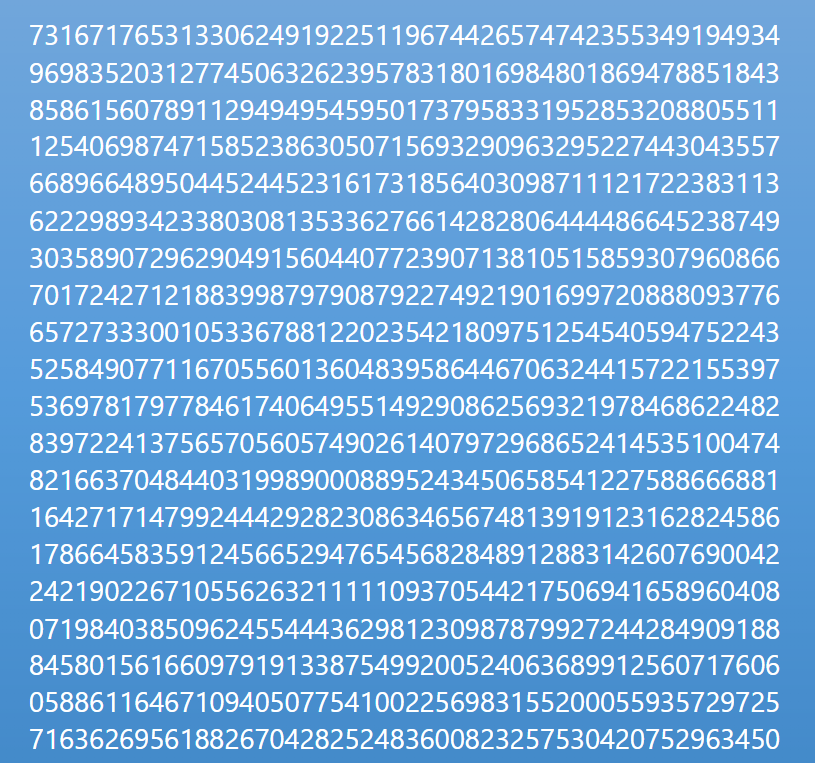
\includegraphics[width = 0.8\textwidth]{../pic/3/3.0.png}
\end{figure}

\section{3.2 思路分析}

题目本身很简单,解决和验证思路可以分为三部分
\begin{enumerate}
    \item \textbf{数据输入}. 
        \begin{itemize}
            \item 题中要求从文件输入,我们将数据存放在input文件夹的input3.txt中;
            \item 考虑到数据的长度,只能以字符串的形式输入,并通过Problem1中提到过的库函数以数组的方式处理数据。
        \end{itemize}
    \item \textbf{算法设计}. 只需要从第[0……n-1]位开始向后逐位扫描即可,但考虑到n位数相乘可能大于int甚至long类型的边界,综合
        考虑并查阅资料后,决定采用\lstinline{Math}库里的\lstinline{BigInteger}这个类. 下面对未采用的优化方案做出解释。
        \begin{itemize}
            \item 高精度. 即用\lstinline{String}模拟高位数乘法的过程。而实际上\lstinline{BigInteger}类已经帮我们内部实现了这一点,
                而且配有丰富的函数和数值优化,这一定是比我们自己写更快更方便的。
            \item 记忆组中的最小值,如果下一个比这个小就可以直接跳过。这一步看似优化了一步,实际上增加了比较的环节,从算法复杂性分析来看
                并没有优化。
        \end{itemize}
    \item \textbf{数据测试}. 本题思路简单,用题中所给数据验证即可
\end{enumerate}

\section{3.3 代码展示}

为了便于验证,用一个循环来模拟不断查询新的最大子序列

\lstinputlisting[
    language = Java,
    caption = {\bf Problem3.java}
    ]{../../../ProblemSet/src/Problem3.java}

\section{3.4 结果展示}

输入数据采用题目中的“1000位数据”,并设置三种长度

\begin{figure}[H]
    \centering
    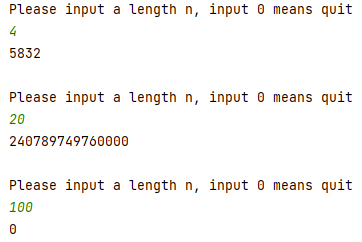
\includegraphics[width = 0.4\textwidth]{../pic/3/3.1.png}
\end{figure}

\section{3.5 总结与收获}

第一次看到本题时我想到了3.2中所写的一些思路,苦恼于怎么优化其时间复杂度以及优雅地写出来。
并不知道也没有打算使用BigInteger但后来认真分析,查阅JDK的官方文档和BigInteger的实现原理后
意识到BigInteger这个类的便捷性和性能远比自己写的好,

“如果你不知道为什么要优化,那这样的优化毫无意义(not make sense at all)” 

\rightline{—— Professor.Weaver (UC.Berkeley)}
% \include{chapter10}
% \include{chapter11}
% \include{chapter12}

\end{document}